%%Introduction

In this Section, we consider models with a photon, a W boson, a Z boson or a Higgs boson in the final state, 
accompanied by Dark Matter particles that either couple directly to the boson or are mediated by 
a new particle. The experimental signature is identified as \textit{V+MET}. 

These models are interesting both as extensions of models where the gluon provides 
the experimentally detectable signature, 
and as stand-alone models with final states that cannot be generated by the models in
Section~\ref{subsec:MonojetLikeModels}.

%%%Classification of models

%FIXME: CD - the tufte.cls on SVN does not like citep. Why? Will look into it later.
\begin{figure}[h!]
  \centering
    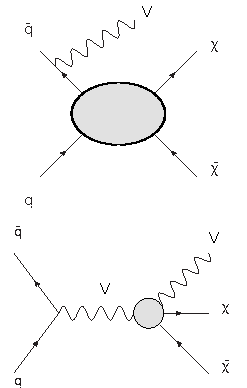
\includegraphics[width=0.5\textwidth]{figures/VPlusMET_EFT}
  \caption{Sketch of EFT models for V+MET searches, adapted from~\citep{Nelson:2013pqa}. \label{fig:VPlusMET_EFT}}
\end{figure}
% 
The models considered can be divided in four categories:
\begin{description}
 \item[EFT models where the boson is radiated from the initial state] As depicted in 
 the top diagram of Figure~\ref{fig:VPlusMET_EFT}, these  models follow the nomenclature and theory 
 for the EFT benchmarks commonly used by MET+X searches~\citep{Goodman:2010ku}. 
 \item[EFT models where the boson is directly coupled to DM] Shown in the bottom of Figure~\ref{fig:VPlusMET_EFT},
 these models allow for an EFT vertex that directly couples the boson to Dark Matter. 
 \item[Simplified models where the boson is radiated from the initial state] These models follow those
 already described in Section~\ref{subsec:MonojetLikeModels}, replacing the initial state gluon with a boson.
 \item[V-specific simplified models] These models postulate direct couplings of new mediators
 to bosons, e.g. they couple the Higgs boson to a new scalar~\citep{Carpenter:2013xra}. 
\end{description}

The following Sections describe the models within these categories, 
the parameters for each of the benchmark models chosen,
the studies towards the choices of the parameters to be scanned, 
and finally point to the location of their Matrix Element 
implementation. 

\paragraph{EFT models with ISR boson radiation}

Searches in the mono-jet final state are generally more sensitive
with respect to final states including bosons, due to the much 
larger rates of jet+MET signal events with 
respect to radiation of bosons~\citep{Zhou:2013fla}, 
in combination with the low branching ratios if leptons from 
boson decays are required in the final state. 
The rates for the Higgs boson radiation is too low for EFT models 
to be considered a viable benchmark~\citep{Carpenter:2013xra}.

However, the presence of photons~\citep{Khachatryan:2014rwa, Aad:2014vka}, 
leptons from W and Z decays~\citep{Khachatryan:2014tva, Aad:2014vka, ATLAS:2014wra} and W or Z bosons decaying hadronically~\citep{Aad:2013oja}
allows to reject the background more effectively, making Z/gamma/W+MET search results for simple EFT benchmarks still worth comparing with jet+MET. 
The three commonly chosen EFT benchmarks for Dirac dark matter that are kinematically distinct for what concerns the observables used in MET+X searches~\footnote{[CD: we would need a plot here, or a reference to monojet section where this is shown]} and span a wide range of MET spectrum in the boson+MET searches are, in the notation of ~\citep{Goodman:2010ku}, the D1 (scalar SM/WIMP interaction), D5 (vector-vector interaction) and D9 (tensor interaction) operator. 

The case for searches with W bosons in the final state is strenghtened by the presence of particular choices of couplings between the WIMP and the up and down quarks which enhance W radiation~\citep{Bai:2012xg}. 
We consider three sample cases for the product of 
Dirac WIMP/down quark and WIMP/up quark couplings $\xi$,
in the case of a vector or axial-vector interaction
\footnote{[CD: refer to VV/AV/VA/AA monojet studies.]}: 
\begin{itemize}
 \item No couplings between WIMP and either up or down quarks~($\xi=0$);
 \item Same coupling between WIMP and each of the quark types~ ($\xi=1$);
 \item Coupling of opposite sign between WIMP and each of the quark types~($\xi=-1$);
\end{itemize}

The $\xi=-1$ case produces constructive interference between the two diagrams in which a W is produced from an initial state of an up and a down quark. This in turn increases the cross-section of the process and the hardness of the spectrum of missing transverse energy or transverse mass used for the searches. The sensitivity of the W+MET search for this benchmark surpasses that of the jet+MET search, as gluon radiation does not distinguish between different couplings scenarios. 

The above considerations lead to the following prioritized list of benchmark models for EFT models with ISR boson radiation: 

\begin{description}
 \item[Vector interaction with vector-vector couplings (D5)]. For both jet+MET and boson+MET searches, the kinematic of this operator corresponds to that of couplings that are vector-axial (D7), axial-axial (D8) and axial-vector (D6). In the case of W boson radiation, the three coupling scenarios $\xi=1,0,-1$ should be investigated. This operator populates the high MET
 \item[Tensor interaction (D9)]. As shown in Figure \textbf{[CD: add picture from Andy]}, this operator populates a higher MET range with respect to the other operators chosen. 
 \item[Scalar interaction (D1)]. This operator has the lowest cross-section and sensitivity at colliders in this final state, as DM production from light quarks via a scalar interaction is suppressed with respect to heavy quarks. However, it has the hardest MET spectrum of the EFT operators chosen, and results obtained using this operator as benchmark may be used for recasting signals with a similarly hard MET distribution.~\footnote{Q for Andy/M-E: ZZchichi max gamma: is it the same kinematics regardless of DM? See fig. 2 of ATLAS monoZ.}
\end{description}

\paragraph{EFT models with direct DM-boson couplings}

A complete list of effective operators with direct DM/boson couplings, 
up to dimension 7, can be found in~\citep{Cotta:2012nj}.

\paragraph{Simplified models with ISR boson radiation}

The choice of simplified models with ISR boson radiation follows both that of the corresponding EFT operators and of the jet+MET models. The primary benchmark model is a vector mediator exchanged in the s-channel~\footnote{[CD: link to the monojet section for diagram]}. Similarly to the EFT case, we recommend to test the three different coupling scenarios for the W+MET signature. \footnote{CD: how do we justify having 3 EFT scenarios and only one simplified model? We have the t-channel colored scalar mediator available from earlier ATLAS mono-Z}.

\paragraph{Specific simplified models}
